
\subsubsection{Raspicontroller}

Der Raspicontroller ist für die Ablaufsteuerung und die Erkennung des Korbes zuständig. Die Applikation ist in Python geschrien und wird als Service auf einem Raspberry Pi ausgeführt. Auf dem Raspberry Pi ist das Betriebssystem Arch Linux installiert. Arch Linux lässt sich ohne grafische Oberfläche betreiben, wodurch wenig Ressourcen verwendet werden. Das Betriebssystem lässt sich komplett über Textdateien konfigurieren. Das ist vor allem nützlich wenn keine grafische Oberfläche vorhanden ist. Mit dem Raspberry Pi wird eine Kamera über eine CSI-Schnittstelle\footnote{Camera Serial Interface} verbunden. Zusätzlich wird ein Wlan-Dongle und das Freedom-Board per USB angeschlossen. Einen Überblick über die angeschlossene Peripherie ist dem Blockdiagramm in Abbildung \ref{fig:blockdiagramm} zu entnehmen. Der Raspberry Pi stellt einen Access Point zu Verfügung, damit man sich mit dem Fotoshoot UI drahtlos verbinden kann. Die Steuerbefehle werden über eine REST-Schnittstelle entgegen genommen. Diese Schnittstelle wird über einen Webserver bereitgestellt. Der Webserver wurde mit Hilfe der Python-Bibliothek \texttt{web.py} erstellt. Detaillierte Angaben zur Schnittstelle kann dem Abschnitt \ref{sec:rest-schnittstelle} entnommen werden. Um den Korb zu erkennen wird ein Foto geschossen und ein Algorithmus erkennt die Position des Korbes. Die Kamera wird mit der Python-Bibliothek \texttt{picamera} angesteuert. Diese Bibliothek liefert das Bild als Python-Objekt zurück, welches danach direkt dem Algorithmus übergeben werden kann. Der Algorithmus wurde selbst entwickelt und in Python implementiert. Abbildung \ref{fig:ablauf-ortung-des-korbes-algorithmus} zeigt grob den Ablauf des Algorithmus.

\begin{figure}[h!]
\centering
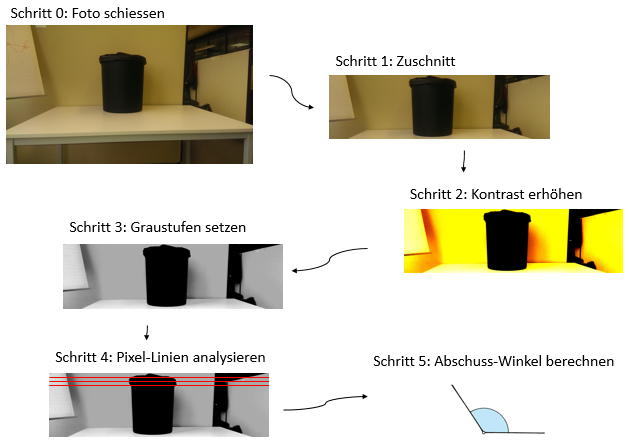
\includegraphics[width=0.7\linewidth]{../../fig/ablauf-ortung-des-korbes-algorithmus}
\caption{Ablauf Erkennung des Korbes}
\label{fig:ablauf-ortung-des-korbes-algorithmus}
\end{figure}

Die Position des Korbes wird als Anzahl Schritte über das Freedom-Board an den Schrittmotor weitergeleitet. Mit dem Freedom-Board wird über eine serielle Schnittstelle kommuniziert. Die serielle Schnittstelle wird mit der Python-Bibliothek \texttt{pyserial} angesteuert. Detaillierte Angaben zur Schnittstelle kann dem Abschnitt \ref{sec:schnittstelle-raspi-freedom} entnommen werden.